ATLAS (\textbf{A} \textbf{T}oroidal \textbf{L}HC \textbf{A}pparatu\textbf{S}) is a 
multi-purpose particle detector located at one of the 
LHC interaction points 100 meters underground. 
It is the largest particle detector ever built with a weight of about 7000 tonnes, a length of 44 m, 
and a diameter of 25 m as shown in Figure~\ref{fig:exp.atlas.atlas}.
It is designed to probe Higgs physics, QCD, and flavour physics, as well as a multitude of beyond the Standard Model (BSM) physics scenarios including 
supersymmetry.

ATLAS covers a solid angle of almost $4\pi$ to capture as much information from the collisions 
as possible. 
It is composed of multiple layers of detectors to ensure that all particles produced in the 
collision are identified and measured with high accuracy.
These subsystems are shown in Figure~\ref{fig:exp.atlas.atlas}.
The first detector resides in the part closest to the
LHC pipe and is composed of silicon tracking sensors designed to reconstruct the paths
of charged particles. 
Next, comes the electromagnetic and hadronic calorimeter cells that 
measure the energy of particles. Last comes the muon spectrometer in the outermost part of the 
detector to detect muons since they penetrate the calorimeters. 
An axial magnetic field of 2 T is applied across the inner detector while a toroidal magnetic field 
of approximately 0.5 T is applied across the muon detectors.
The remainder of this chapter will describe in more details these detectors.




\begin{figure}[t!]
\centering
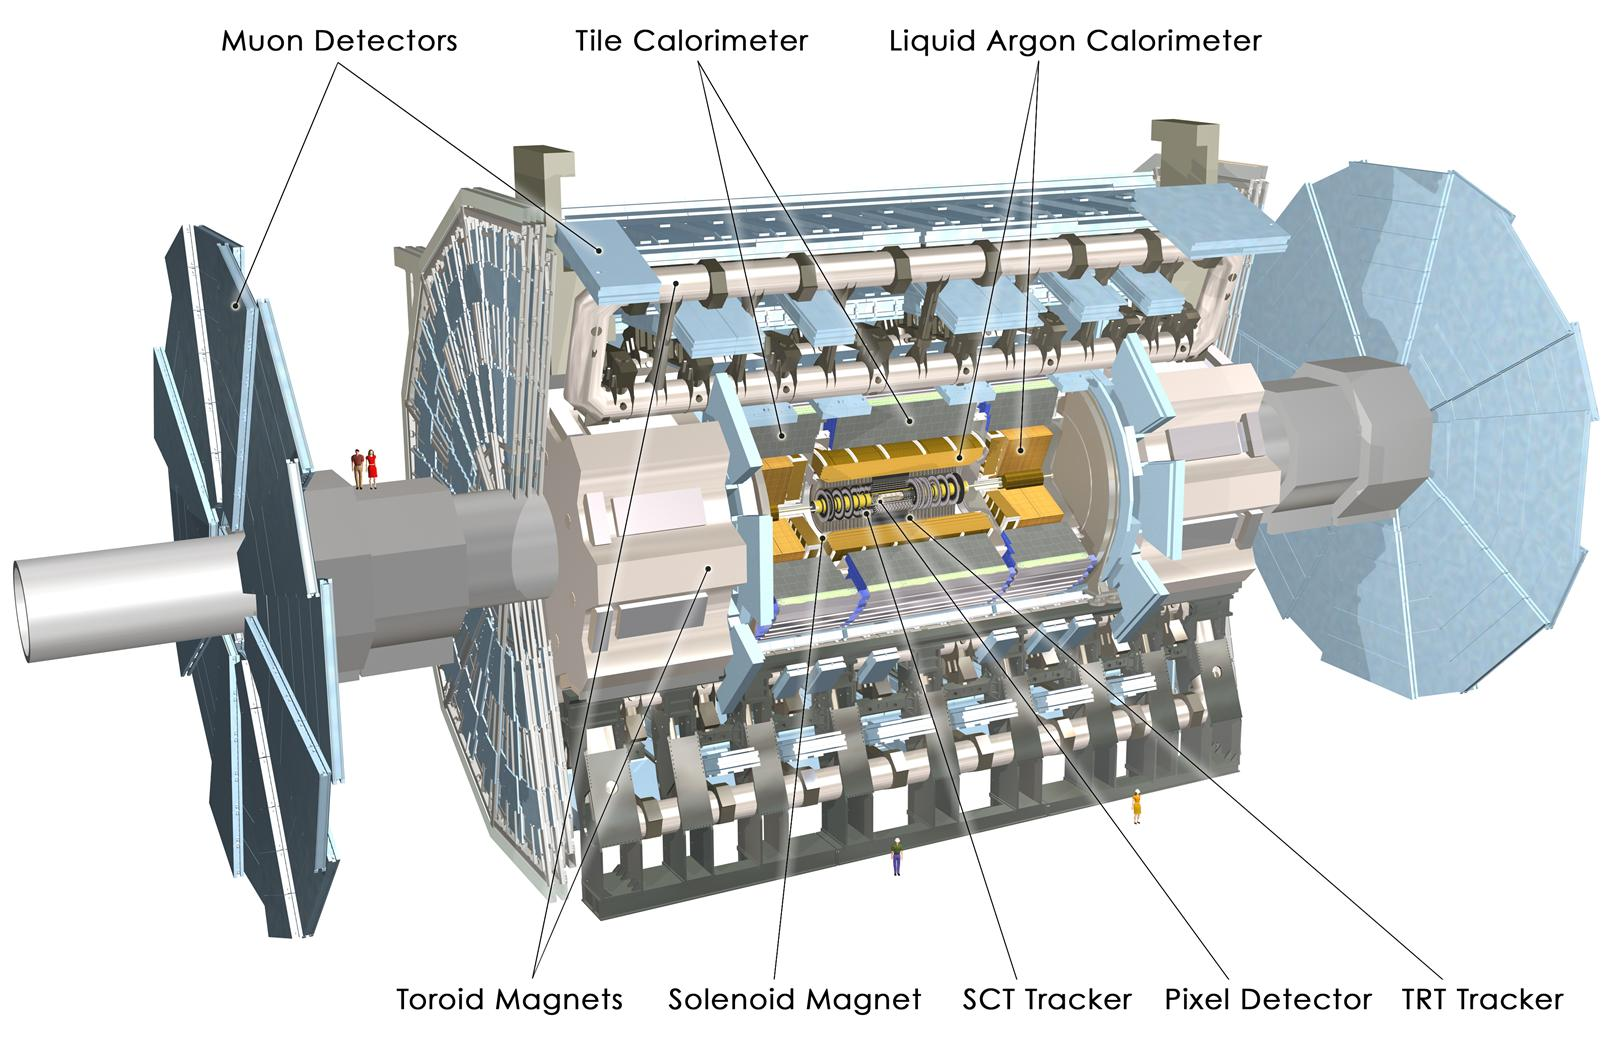
\includegraphics[width=0.95\textwidth]{all_atlas.jpeg}
\caption{Overview of all the subsystems of the ATLAS detector.}% cite??
\label{fig:exp.atlas.atlas}
\end{figure} 




\subsection{Co-ordinate System}

The common coordinate system of ATLAS is right-handed Cartesian, 
with its origin at the nominal interaction point. 
The axes are oriented such that the $x$-axis is pointing towards the center of the LHC ring, the $y$-axis is directed
vertically upward, and the $z$-axis defines one of the beam directions.
The $(x, y)$ plane defines the transverse plane, usually represented by polar coordinates $(r,\phi)$
with $\phi=0$ on the $x$-axis.
The polar angle $\theta$ is replaced by the pseudorapidity
\begin{equation}
\eta = - \ln\left(\tan\left(\frac{\theta}{2}\right)\right),
\end{equation}
shown in Figure~\ref{fig:exp.atlas.pseudo}.
It is named after the rapidity ($y$) since it yields the same quantity for massless particles
\begin{equation}
y = \frac{1}{2}\ln\left(\frac{E+p_Z}{E-p_Z}\right),
\end{equation}
which is invariant under boosts in the $z$-direction.
It is common to describe the separation between two physical objects in the detector by 
\begin{equation}
\Delta R = \sqrt{\Delta \eta^2 + \Delta \phi^2}
\end{equation}

\begin{figure}[htb!]
\centering
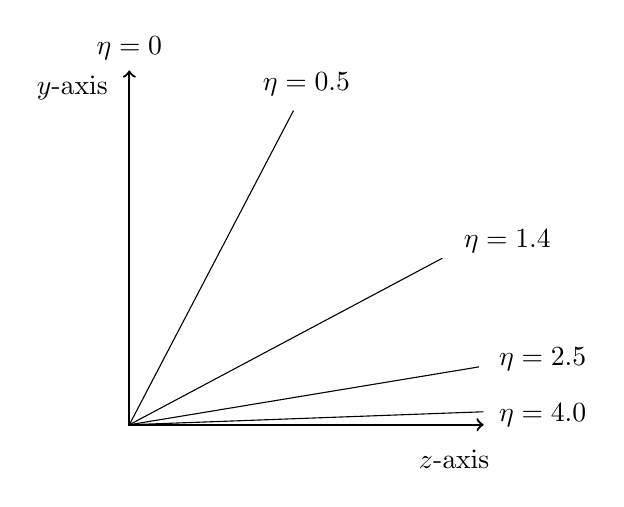
\begin{tikzpicture}[scale=1.5]
    % Draw axes
    \draw [<->,thick] (0,3) node (yaxis) [above] {$\eta=0$}
        |- (3,0) node (xaxis) [right] {}; %$\eta = \infty$
    % Draw two intersecting lines
    \draw (0,0) coordinate (a_1) -- (2.65,1.41) coordinate (a_2);
    \draw (0,0) coordinate (b_1) -- (2.96,0.49) coordinate (b_2);
    \draw (0,0) coordinate (c_1) -- (1.39,2.66) coordinate (c_2);
    \draw (0,0) coordinate (d_1) -- (2.998,0.11) coordinate (d_2);
    \draw (3.5,0.375) node[above]      
      {$\eta = 2.5$};
    \draw (3.2,1.375) node[above]      
      {$\eta = 1.4$};
    \draw (1.5,2.7) node[above]      
      {$\eta = 0.5$};
    \draw (3.5,-0.1) node[above]      
      {$\eta = 4.0$};
    \draw (2.75,-0.45) node[above]      
      {$z$-axis};
    \draw (-0.1,2.85) node[left]      
      {$y$-axis};
\end{tikzpicture}
\caption{Illustration of some pseudorapidity values relevant for ATLAS.}
\label{fig:exp.atlas.pseudo}
\end{figure} 

\subsection{Inner detector}

In the innermost part of ATLAS is placed a tracking detector referred to as the Inner Detector (ID). 
It has finely segmented detectors to reconstruct the tracks of charged particles in the magnetic field of the solenoid.
The main subsystems of the ID are the pixel detector, the SemiConductor Tracker (SCT), and the Transition Radiation Tracker (TRT)
shown in Figure~\ref{fig:exp.atlas.id.all}.
Overall these give coverage of the solid angle defined
by $|\eta| < 2.5$, and occupy the volume with $33.25 < r < 1082$ mm. Using these systems,
its purpose is to detect the path taken by charged particles as they bend through the
magnetic field, and hence determine their momenta.
Particles from the main $pp$ interaction pass through several layers of silicon detectors each providing a 2-dimensional coordinate. 
To reduce correlations between individual points the layers are spread out evenly along the tracks.
Figure~\ref{fig:exp.atlas.id.rad} shows a charged particle with 10 \GeV~transverse momentum, denoted by \pt, that
emerges from the interaction point and traverses the beam-pipe, four pixel layers, 
four double layers of SCT sensors, and around 35 TRT straws.
These elements will be described next.

\begin{figure}[htb!]
\centering
\includegraphics[width=0.95\textwidth]{id.jpg}
\caption{Overview of the subsystems of the inner detector of ATLAS.}
\label{fig:exp.atlas.id.all}
\end{figure}

\begin{figure}[htb!]
\centering
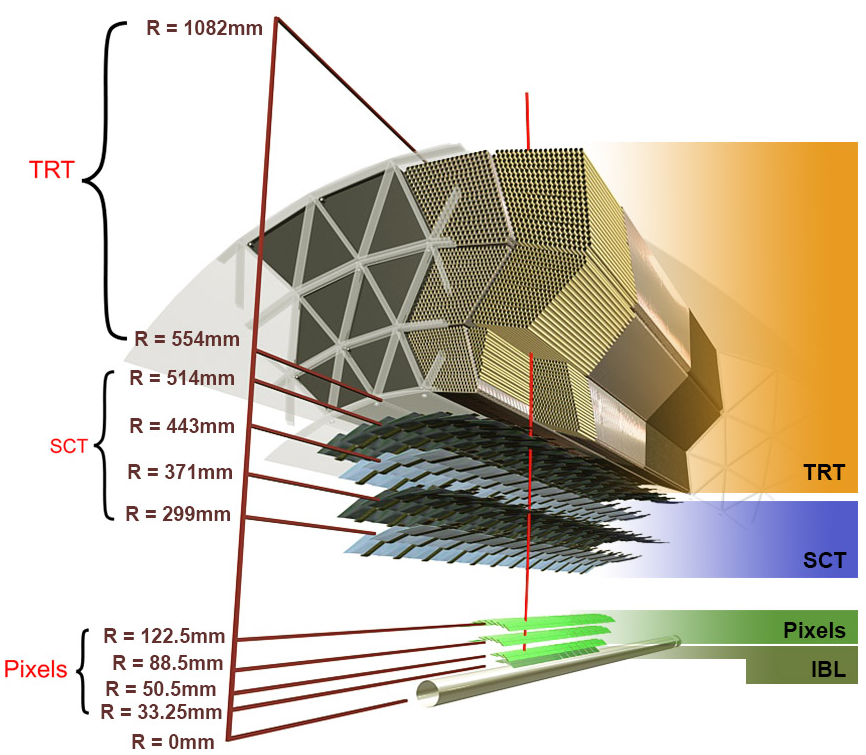
\includegraphics[width=0.85\textwidth]{id_ibl.png}
\caption{Drawing showing the detector elements crossed by a charged particle with 10 \GeV~\pt
in the barrel of the Inner Detector. The particle emerges from the interaction point and traverses the beam-pipe, 
one IBL layer, three pixel layers, four double layers of SCT sensors, and around 35 TRT straws.}
\label{fig:exp.atlas.id.rad}
\end{figure}

\subsection*{Pixel detector}
Since the pixel detector is the closest to the beam pipe ($33.25 < r <242$ mm), it is
the highest resolution detector. It contains 140 million semiconductor pixels each of just
50 $\times$ 400 $\mu$m, 
thus giving a 2-dimensional coordinate with just one layer. The best resolution is in the $\varphi$ coordinate. 
As a result, it is able to measure the charged particle track intersection 
position at the different layers  up
to a precision of 10 $\times$ 115 $\mu$m.
This resolution is important since the 
the area subtended by a given solid angle is at its smallest value near the interaction point.
 It is also designed to tolerate the very high radiation
doses that it is exposed to at such proximity to the interaction point. The detector is
formed of three barrel layers as well as two end-cap structures. Each of the end-caps
comprises four discs of sensors, arranged such that most tracks are more likely to hit pixels in at
least three distinct layers.
The pixel detectors provide the position of the main $pp$
interaction, called the primary vertex, and subsequent vertices from 
$B$-meson decays. These are important parameters for the identification of jets originating from $b$-hadrons,
essential for most of the physics program of ATLAS, including the search presented in this dissertation. 
 Further details can be found in the corresponding technical design report [8].


\subsection*{SCT}

The SCT surrounds the pixel layers.
The SCT is formed of four stereo layers in the barrel,
along with nine discs in each end-cap. 
Each SCT layer is composed of a double layer of silicon
strips, whose axes are tilted by 40 mrad with respect to one another. The pair of measurements at
each SCT layer locates charged particles in $r - \phi$ with an accuracy of 17 $\mu$m, 
and along $z$, with an accuracy of 580 $\mu$m.
The SCT provides between four and nine measurements per particle, with
coverage up to $|\eta|=2.5$.
Further details can be found in the technical design report of the inner
detector [9, 10].

         
\subsection*{TRT}

The TRT is the largest of the sub-detectors in the ID.
It is composed of  $\sim$300,000 straw drift tubes 
that provide position measurements with an accuracy of $\sim$130 $\mu$m in $\phi$.
A large number of hits, around 35 per particle, is provided, with coverage up to
$|\eta|$=2.0. 
It operates based on the ionization of the gas inside the tubes (70\% Xe, 27\% CO2 and 3\% O2) 
when traversed by charged particles; the ions then drift radially due to
the potential difference, and the excess charge is collected and detected. 
The tubes are arranged parallel to the beam axis in the barrel region, and radially in the end-caps. 
In addition to providing particle tracks, 
the TRT also provides particle identification through
the detection of transition radiation\footnote{Transition radiation is emitted whenever a charged particle 
crosses the boundary between two media.}. For example, 
electrons will emit more transition radiation photons than charged hadrons.


\subsection{Calorimeters}


The calorimeter system measures the energy of hadrons, electrons and photons.
The ATLAS calorimeter is divided into an electromagnetic calorimeter based on liquid argon (LAr)
and a hadronic calorimeter based on  iron-scintillator ``tiles'' (Tile).
The distinction is due to the
different interaction behaviour between the calorimeter and electrons/photons on one side and hadrons on the other side. 
 [12].
An overview of the calorimeter system can be seen in Figure~\ref{fig:exp.atlas.calo}. 
Overall they cover solid angles up to $|\eta| < 4.9$, with the electromagnetic calorimetry providing finer 
grained measurements to augment the inner detector for electron and photon measurements, while
the hadronic calorimeter is coarser but sufficient for jet reconstruction and measurements
of missing transverse momentum.

The ATLAS calorimeters are sampling calorimeters. 
Incident particles produce showers of energy in the calorimeter. 
Only a fraction of the energy produced by the particle is
measured by active detector sensors. 
The energy of the full shower can be inferred from the observed
energy. Thus a calibration must be used to estimate the true energy
of any observed shower in the calorimeter. Each calorimeter is also segmented in $\eta$ and
$\phi$  to provide some directional information, although it is coarser than that from
the inner detector. Finally, the calorimeter is designed to limit ``punch-through'' of high
energy jets into the muon chambers.

\begin{figure}[htb!]
\centering
\includegraphics[width=0.95\textwidth]{calo.jpg}
\caption{Overview of the different calorimeters in ATLAS.}% cite??
\label{fig:exp.atlas.calo}
\end{figure} 


\subsection*{LAr Calorimeters}

The energies of electrons and photons are measured by the LAr electromagnetic calorimeters composed of 
the barrel section with $|\eta| <$ 1.475, and end-cap sections with $1.375 < |\eta| < 3.2$.
These detectors provide complete $\phi$ coverage and fast readout, in addition to 
high granularity measurements, critical for particle identification in the range $|\eta|<2.5$
There is a region of slightly degraded performance where the barrel and end-cap sections 
do overlap. Most ATLAS analyses, including the one presented in this dissertation, ignore
electron and photon candidates that fall into this ``crack'' region.
Figure~\ref{fig:exp.atlas.accordion}
shows a cut-away of the different layers in the electromagnetic barrel calorimeter. The first layer, referred to as
the ``strips'', provides very fine segmentation in $\eta$. The strips can separate between showers initiated
by electrons or photons and showers initiated by neutral pions. The second sampling provides most
of the energy measurement and has fine segmentation in both $\eta$ and $\phi$. The third sampling is coarser
and adds additional depth to the calorimeter.



\begin{figure}[htb!]
\centering
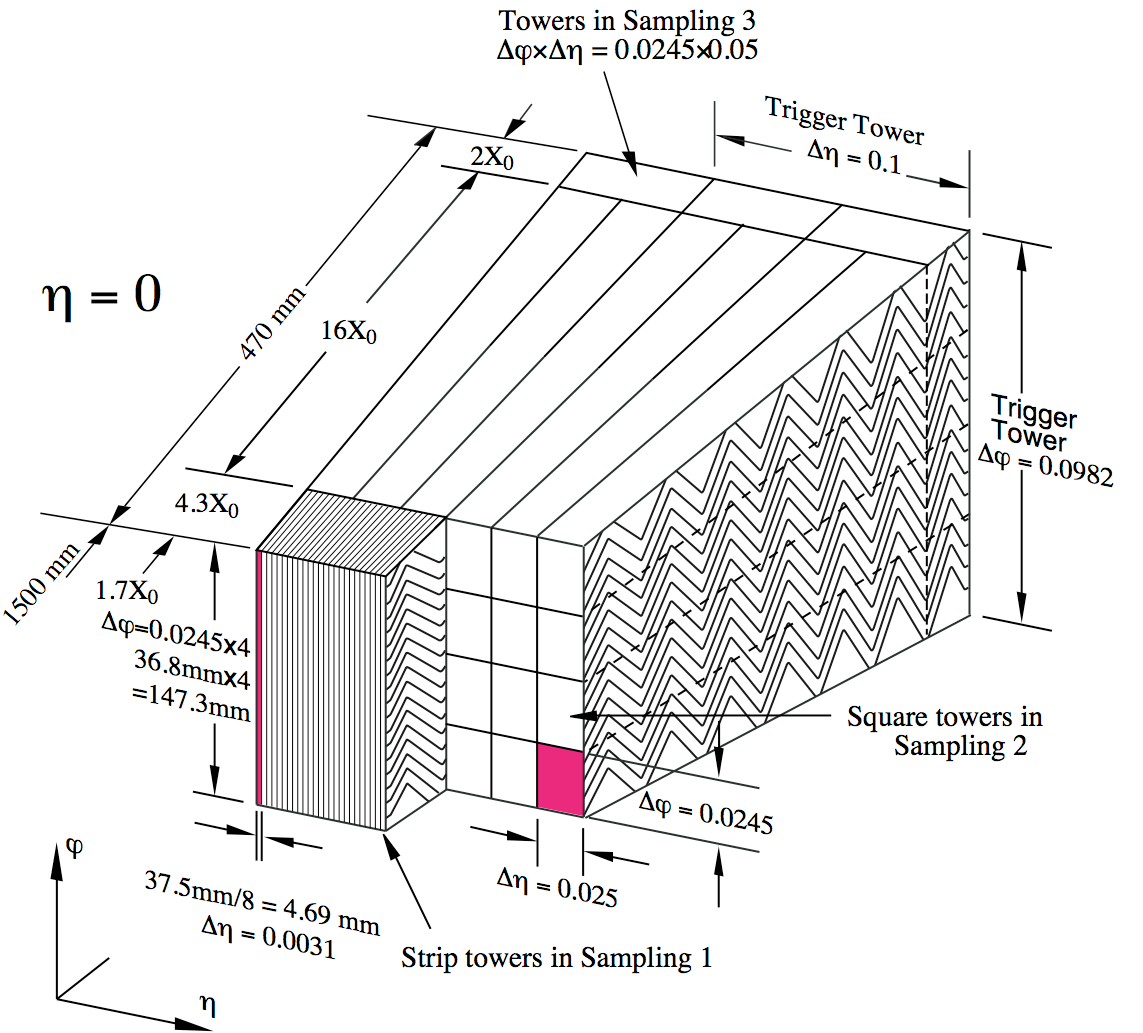
\includegraphics[width=0.75\textwidth]{accordion}
\caption{Sketch of the accordion structure of the LAr EM calorimeter
where the different layers are clearly visible. 
The granularity in $\eta$ and $\phi$ of the cells of each of the three layers is shown.}% cite??.}
\label{fig:exp.atlas.accordion}
\end{figure} 


\subsection*{Tile Calorimeters}

The tile calorimeter is the hadron calorimeter covering the range of $|\eta| < 1.7$.
%where the LAr hadronic calorimeter takes over.
The tile calorimeter uses steel tiles as an absorber and scintillating tiles as the detector.
The scintillator tile calorimeter is separated into a barrel and two extended barrel cylinders.
The light produced in the scintillators is read out with wavelength-shifting optical fibers to photomultipliers (PMTs) placed on the outside of the calorimeter. 
%The fibres absorb the blue light from the scintillators and reemit it at longer wavelengths where it reaches the photomultipliers through total reflection inside the fibres. 


\subsection{Muon System}

The ATLAS muon system is used as a trigger to select events with high energy muons and to measure the position of muons
as they traverse the detector.


The system covers the range of $|\eta| < 2.7$ and operates on the principle of measuring the deflection of tracks due to magnetic fields.
There is then a magnetic field in the barrel section, $|\eta| < 1.4$, induced by the main barrel coils, 
and a magnetic field in the end-cap region, $1.6 < |\eta| < 2.7$, induced by separate end-cap coils, as can be 
seen in Figure~\ref{fig:exp.atlas.muon.all}.
In the region $1.4 < |\eta| < 1.6$, the bending will occur by a combination of the barrel and end-cap fields.

Several technologies are used to select the events and make measurements.
The barrel region has resistive-plate chambers (RPC) for $|\eta| < 1.05$  that provide very fast timing information, $\sim 10$ ns,
used for triggering. The barrel also has monitored drift tubes (MDT) for $|\eta| < 2.0$ that give precise measurements, $\sim 35 \mu$m per chamber,
in the $\left(\eta,z\right)$-plane where the bending occurs.
The forward region of the detector, $2.0 < |\eta| < 2.7$,  has Cathode strip detectors (CSCs)  nearest to the interaction point,
followed by thin-gap chambers (TGCs) and additional MDTs. The CSCs achieve a resolution of 40$\mu$m in the $\left(\eta,z\right)$-plane
and 5 mm in the transverse plane.
The layout of these components is more clearly shown in Figure~\ref{fig:exp.atlas.muon}.


\begin{figure}[htb!]
\centering
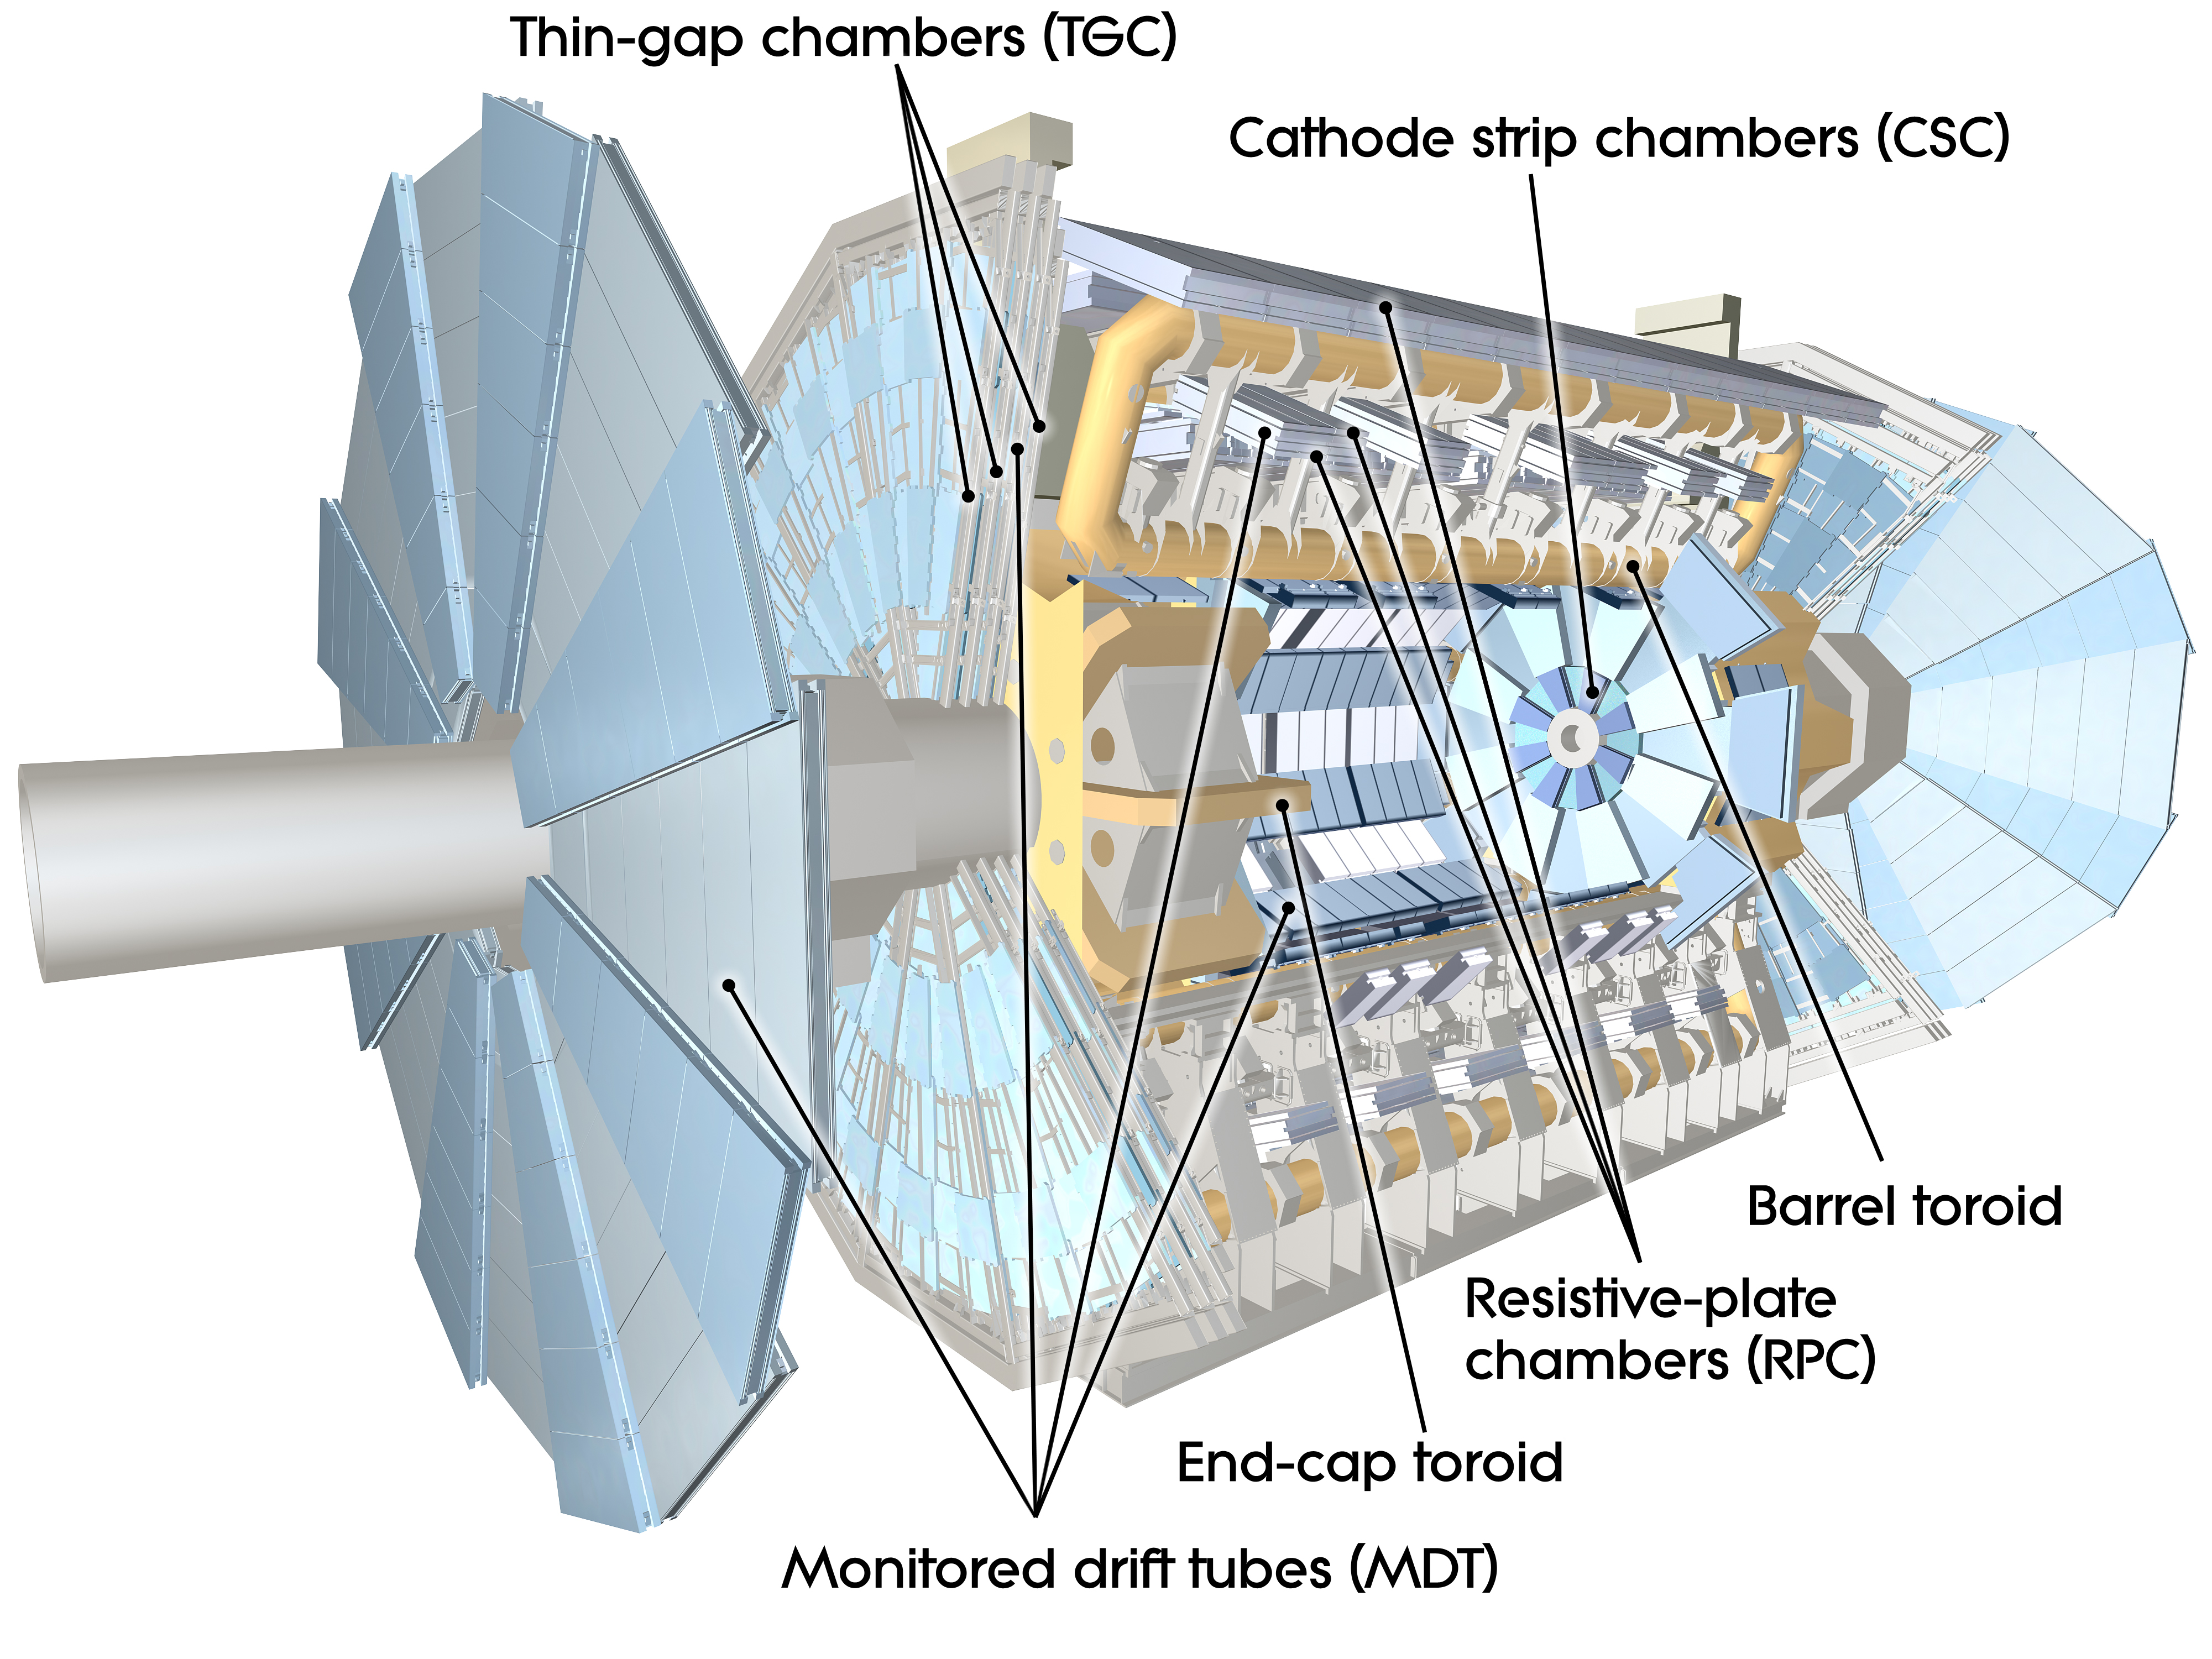
\includegraphics[width=0.95\textwidth]{muon}
\caption{Overview of the ATLAS muon system.}% cite??.}
\label{fig:exp.atlas.muon.all}
\end{figure} 


\begin{figure}[htb!]
\centering
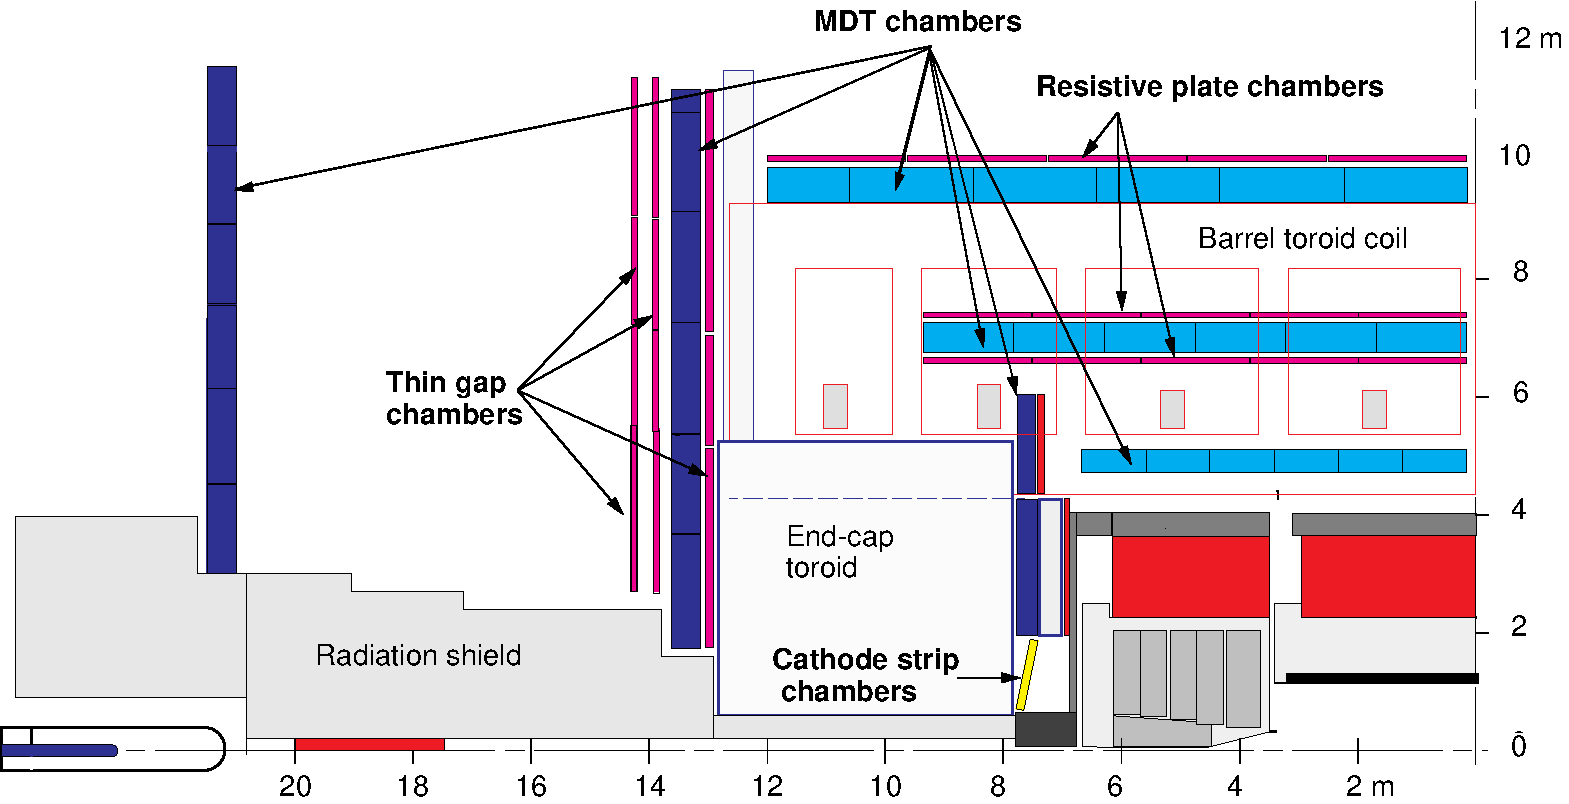
\includegraphics[width=0.95\textwidth]{muon-atlas}
\caption{Cross-sectional view of the muon detectors of ATLAS in the $\left(y-z\right)$-plane.}% cite??.}
\label{fig:exp.atlas.muon}
\end{figure} 
